% =====================================================================
%  Chapter 1 — The Cosmic Budget
% =====================================================================

\chapter{The Cosmic Budget}
\label{ch:budget}

The first question is not what dark matter is. It is how much of it there is,
measured in a way that does not depend on any model of what it might be. The
answer has been stable for a decade, it is known to a few parts in a thousand,
and everything else in this book is commentary on that number.

\section{The number}The reference measurement remains the Planck 2018 analysis of the cosmic
microwave background, published in 2020 and still the baseline against which
new results are compared \idx{Planck Collaboration}. Planck fixes a set of
parameters that add up to the universe:

\begin{itemize}
\item Cold dark matter density: $\Omega_c h^2 = 0.1200 \pm 0.0012$.
\item Baryon density: $\Omega_b h^2 = 0.0224 \pm 0.0001$.
\item Hubble constant: $H_0 = 67.36 \pm 0.54\ \kms$.
\item Matter fraction: $\Omega_m \approx 0.315$.
\item Dark energy fraction: $\Omega_\Lambda \approx 0.6847$.
\item Fluctuation amplitude: $\sigma_8 = 0.811$.
\end{itemize}

Dividing through gives the familiar picture. Of the total energy density of
the universe, about 68.5 per cent is dark energy, about 26.8 per cent is dark
matter, and about 4.9 per cent is ordinary matter. Set against matter
alone --- the part that can clump into galaxies --- dark matter is 84 per
cent. That ratio is the reason the subject exists at all: ordinary matter is
a minority component of the universe, and dark matter is what the majority of
the gravitating universe is made of.

\begin{figure}[!htbp]
\centering
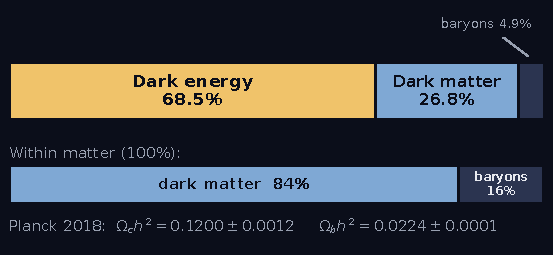
\includegraphics[width=\textwidth]{../figures/fig_budget.pdf}
\caption{The cosmic energy budget as fixed by Planck 2018, expressed as
fractions of the total. Dark matter and dark energy together are 95.3 per
cent of everything; ordinary matter is the small remainder. Within matter,
dark matter is 84 per cent by mass.}
\label{fig:budget}
\end{figure}

\figref{fig:budget} shows the division. The proportions are not a
schematic or an illustration; they are the output of a likelihood analysis
whose principal parameters are the ones listed above.

\section{Why the CMB measures this directly}The reason the number is so precise is structural rather than
accidental. The universe at recombination was a photon-baryon fluid with
dark matter providing gravitational wells. Dark matter does not interact
electromagnetically, so it does not participate in the photon-baryon acoustic
oscillation --- it only provides the potential wells in which the fluid
oscillates. The spacing of the acoustic peaks in the CMB temperature and
polarisation spectra therefore measures the dark matter density with a
directness that galaxy surveys cannot match: the third peak's position is a
function of $\Omega_c h^2$ and essentially nothing else.

Three further features of the same data make the measurement robust. The
\emph{baryon loading} of the peaks --- the relative heights of the odd and
even peaks --- fixes $\Omega_b h^2$ separately, so that the two densities are
measured rather than traded against each other. The \emph{damping tail} at
small angular scales probes free streaming and therefore constrains the
mass of any dark matter particle that is light enough to behave as a
cosmological fluid rather than a pressureless one. And the \emph{lensing
signal} in the Planck CMB maps measures the growth of structure between
recombination and the present, which closes the loop on the same density
from a completely different physical argument.

The consequence is worth stating plainly, because it is the fact on which the
rest of the book rests: the density of dark matter is known about as well as
the density of ordinary matter, and both are known far better than the
properties of dark matter itself.

\section{What ``dark'' means}``Dark'' is a statement about interaction channels, not about
appearance. The constraint is the photon budget. Stars and gas emit and
absorb light; dark matter, whatever it is, does not. The corresponding
constraints are severe and cheap to state: dark matter contributes no
meaningful fraction of the optical emission of any galaxy, of the X-ray
emission of any cluster, or of the thermal emission of any object. It is not
merely faint; it is electromagnetically inert to a degree that no ordinary
matter can imitate, which is why the Bullet Cluster in Chapter~\ref{ch:bullet}
is so decisive.

The word ``cold'' in ``cold dark matter'' refers to something narrower. It
means that the dark matter has been effectively pressureless since
recombination, so that it clusters like a collisionless fluid on scales far
smaller than the acoustic horizon. The qualifier is a hypothesis about
thermal history, not an observation, and Chapter~\ref{ch:ultralight} takes the
case for warm and wave dark matter seriously precisely because it is the
weakest link in the chain.

\section{The local density, and why its convention matters}There is one number in this subject that is quoted
more often than any other and that is not a measurement of the universe at
all. It is the density of dark matter in the neighbourhood of the Solar
System, $\rho_0$, and it is the conversion factor between a laboratory
cross section and the number of events a detector will see.

The convention in use is roughly $\rho_0 = 0.3\ \GeVcmthree$ in the Particle
Data Group review of dark matter searches \idx{Particle Data Group}, and
roughly $0.4$ to $0.45\ \GeVcmthree$ in the axion literature, where the
higher value is used for microwave-re cavity experiments. The discrepancy is
not an error but a difference in the halo model being assumed, and it has
concrete consequences: a limit quoted at $\rho_0 = 0.4$ is roughly 25 per
cent stronger than the same limit quoted at $\rho_0 = 0.3$ when rescaled to a
common convention.

\begin{table}[H]
\centering
\caption{The cosmic energy budget, and the conventions attached to it.}
\label{tab:budget}
\begin{tabular}{@{}>{\RaggedRight\arraybackslash}p{0.40\textwidth}r r@{}}
\toprule
\textbf{Component} & \textbf{Value} & \textbf{Share} \\
\midrule
Dark energy & $\Omega_\Lambda = 0.6847$ & 68.5\% \\
Dark matter & $\Omega_c h^2 = 0.1200 \pm 0.0012$ & 26.8\% \\
Baryons & $\Omega_b h^2 = 0.0224 \pm 0.0001$ & 4.9\% \\
\midrule
Dark matter as a fraction of matter & --- & 84.0\% \\
Local dark matter density (PDG convention) & $\rho_0 = 0.3\ \GeVcmthree$ & --- \\
Local dark matter density (axion convention) & $\rho_0 = 0.4$--$0.45\ \GeVcmthree$ & --- \\
\bottomrule
\end{tabular}
\end{table}

\tabref{tab:budget} collects the budget and the two conventions that
frequently get mixed. The rule this book follows, and the rule that should
be followed in any comparison of limits from different experiments, is simple:
whenever a limit is compared with another, both are rescaled to a single
stated value of $\rho_0$, and the value is printed next to the limit.

\section{What the budget does not tell you}Knowing the density constrains the candidate space without
identifying anything in it. A particle of any mass with the right
interaction strength will do; a population of primordial black holes will
do; an ultralight boson will do. The density also sets the pressure that
every production mechanism must explain, which is the subject of
Part~\ref{part:origins}. But it is worth being explicit about the trap here,
because it recurs in every popular account of the subject: the precision of
$\Omega_c h^2$ is a statement about how well we know how much there is, not
about how well we know what it is.

\begin{keytakeaways}
\item Dark matter is 26.8 per cent of the universe's energy density and
84 per cent of its matter, fixed at $\Omega_c h^2 = 0.1200 \pm 0.0012$ by
the CMB acoustic peaks.
\item The precision of that number comes from structure in the photon-baryon
fluid, which makes it a near-direct measurement rather than an inference from
galaxy dynamics.
\item ``Dark'' is a statement about interaction channels: dark matter is
electromagnetically inert to a degree no ordinary matter reproduces.
\item The local density $\rho_0$ is a convention, not a universal
measurement, and every limit in this book is quoted with the convention it
was published under.
\end{keytakeaways}
